\documentclass[twoside]{book}

% Packages required by doxygen
\usepackage{fixltx2e}
\usepackage{calc}
\usepackage{doxygen}
\usepackage[export]{adjustbox} % also loads graphicx
\usepackage{graphicx}
\usepackage[utf8]{inputenc}
\usepackage{makeidx}
\usepackage{multicol}
\usepackage{multirow}
\PassOptionsToPackage{warn}{textcomp}
\usepackage{textcomp}
\usepackage[nointegrals]{wasysym}
\usepackage[table]{xcolor}

% Font selection
\usepackage[T1]{fontenc}
\usepackage[scaled=.90]{helvet}
\usepackage{courier}
\usepackage{amssymb}
\usepackage{sectsty}
\renewcommand{\familydefault}{\sfdefault}
\allsectionsfont{%
  \fontseries{bc}\selectfont%
  \color{darkgray}%
}
\renewcommand{\DoxyLabelFont}{%
  \fontseries{bc}\selectfont%
  \color{darkgray}%
}
\newcommand{\+}{\discretionary{\mbox{\scriptsize$\hookleftarrow$}}{}{}}

% Page & text layout
\usepackage{geometry}
\geometry{%
  a4paper,%
  top=2.5cm,%
  bottom=2.5cm,%
  left=2.5cm,%
  right=2.5cm%
}
\tolerance=750
\hfuzz=15pt
\hbadness=750
\setlength{\emergencystretch}{15pt}
\setlength{\parindent}{0cm}
\setlength{\parskip}{3ex plus 2ex minus 2ex}
\makeatletter
\renewcommand{\paragraph}{%
  \@startsection{paragraph}{4}{0ex}{-1.0ex}{1.0ex}{%
    \normalfont\normalsize\bfseries\SS@parafont%
  }%
}
\renewcommand{\subparagraph}{%
  \@startsection{subparagraph}{5}{0ex}{-1.0ex}{1.0ex}{%
    \normalfont\normalsize\bfseries\SS@subparafont%
  }%
}
\makeatother

% Headers & footers
\usepackage{fancyhdr}
\pagestyle{fancyplain}
\fancyhead[LE]{\fancyplain{}{\bfseries\thepage}}
\fancyhead[CE]{\fancyplain{}{}}
\fancyhead[RE]{\fancyplain{}{\bfseries\leftmark}}
\fancyhead[LO]{\fancyplain{}{\bfseries\rightmark}}
\fancyhead[CO]{\fancyplain{}{}}
\fancyhead[RO]{\fancyplain{}{\bfseries\thepage}}
\fancyfoot[LE]{\fancyplain{}{}}
\fancyfoot[CE]{\fancyplain{}{}}
\fancyfoot[RE]{\fancyplain{}{\bfseries\scriptsize Generated by Doxygen }}
\fancyfoot[LO]{\fancyplain{}{\bfseries\scriptsize Generated by Doxygen }}
\fancyfoot[CO]{\fancyplain{}{}}
\fancyfoot[RO]{\fancyplain{}{}}
\renewcommand{\footrulewidth}{0.4pt}
\renewcommand{\chaptermark}[1]{%
  \markboth{#1}{}%
}
\renewcommand{\sectionmark}[1]{%
  \markright{\thesection\ #1}%
}

% Indices & bibliography
\usepackage{natbib}
\usepackage[titles]{tocloft}
\setcounter{tocdepth}{3}
\setcounter{secnumdepth}{5}
\makeindex

% Hyperlinks (required, but should be loaded last)
\usepackage{ifpdf}
\ifpdf
  \usepackage[pdftex,pagebackref=true]{hyperref}
\else
  \usepackage[ps2pdf,pagebackref=true]{hyperref}
\fi
\hypersetup{%
  colorlinks=true,%
  linkcolor=blue,%
  citecolor=blue,%
  unicode%
}

% Custom commands
\newcommand{\clearemptydoublepage}{%
  \newpage{\pagestyle{empty}\cleardoublepage}%
}

\usepackage{caption}
\captionsetup{labelsep=space,justification=centering,font={bf},singlelinecheck=off,skip=4pt,position=top}

%===== C O N T E N T S =====

\begin{document}

% Titlepage & ToC
\hypersetup{pageanchor=false,
             bookmarksnumbered=true,
             pdfencoding=unicode
            }
\pagenumbering{alph}
\begin{titlepage}
\vspace*{7cm}
\begin{center}%
{\Large robot\+\_\+properties\+\_\+bolt }\\
\vspace*{1cm}
{\large Generated by Doxygen 1.8.13}\\
\end{center}
\end{titlepage}
\clearemptydoublepage
\pagenumbering{roman}
\tableofcontents
\clearemptydoublepage
\pagenumbering{arabic}
\hypersetup{pageanchor=true}

%--- Begin generated contents ---
\chapter{robot\+\_\+properties\+\_\+bolt}
\label{index}\hypertarget{index}{}This is the documentation of the {\ttfamily robot\+\_\+fingers} package.

The source code is hosted on \href{https://github.com/open-dynamic-robot-initiative/robot_fingers}{\tt Git\+Hub}. Please also use the issue system there if you have a question or want to report a bug.

For more information, on the Tri\+Finger robot and the general architecture of the software, see also our \href{https://arxiv.org/abs/2008.03596}{\tt paper} on the open-\/source version of the Tri\+Finger robot.

\subsection*{Content }


\begin{DoxyItemize}
\item \hyperlink{md_doc_installation}{Build Instructions}
\item \hyperlink{md_doc_singularity}{About Singularity}
\item \hyperlink{md_doc_getting_started}{Getting Started}
\item \hyperlink{md_doc_hardware_testing}{Tools for Hardware Testing}
\end{DoxyItemize}

\subsection*{Links }


\begin{DoxyItemize}
\item \href{https://github.com/open-dynamic-robot-initiative/robot_fingers}{\tt Git\+Hub Repository}.
\item \href{https://github.com/open-dynamic-robot-initiative/robot_fingers/issues}{\tt Bug Tracker}.
\item This package implements a {\ttfamily Robot\+Driver} for the (Tri-\/)Finger robots based on our \href{https://open-dynamic-robot-initiative.github.io/code_documentation/robot_interfaces/docs/doxygen/html/index.html}{\tt {\ttfamily robot\+\_\+interfaces} package}. 
\end{DoxyItemize}
\chapter{Namespace Index}
\section{Namespace List}
Here is a list of all documented namespaces with brief descriptions\+:\begin{DoxyCompactList}
\item\contentsline{section}{\hyperlink{namespacerobot__properties__solo_1_1gepetto__gui__loader}{robot\+\_\+properties\+\_\+solo.\+gepetto\+\_\+gui\+\_\+loader} }{\pageref{namespacerobot__properties__solo_1_1gepetto__gui__loader}}{}
\end{DoxyCompactList}

\chapter{Hierarchical Index}
\section{Class Hierarchy}
This inheritance list is sorted roughly, but not completely, alphabetically\+:\begin{DoxyCompactList}
\item \contentsline{section}{trifinger\+\_\+simulation.\+action.\+Action}{\pageref{classtrifinger__simulation_1_1action_1_1Action}}{}
\item \contentsline{section}{trifinger\+\_\+simulation.\+collision\+\_\+objects.\+Block}{\pageref{classtrifinger__simulation_1_1collision__objects_1_1Block}}{}
\item \contentsline{section}{trifinger\+\_\+simulation.\+trifinger\+\_\+platform.\+Camera\+Observation}{\pageref{classtrifinger__simulation_1_1trifinger__platform_1_1CameraObservation}}{}
\item \contentsline{section}{trifinger\+\_\+simulation.\+visual\+\_\+objects.\+Cube\+Marker}{\pageref{classtrifinger__simulation_1_1visual__objects_1_1CubeMarker}}{}
\item \contentsline{section}{trifinger\+\_\+simulation.\+gym\+\_\+wrapper.\+data\+\_\+logger.\+Data\+Logger}{\pageref{classtrifinger__simulation_1_1gym__wrapper_1_1data__logger_1_1DataLogger}}{}
\item Env\begin{DoxyCompactList}
\item \contentsline{section}{example\+\_\+pushing\+\_\+training\+\_\+env.\+Example\+Pushing\+Training\+Env}{\pageref{classexample__pushing__training__env_1_1ExamplePushingTrainingEnv}}{}
\item \contentsline{section}{trifinger\+\_\+simulation.\+gym\+\_\+wrapper.\+envs.\+trifinger\+\_\+push.\+Tri\+Finger\+Push}{\pageref{classtrifinger__simulation_1_1gym__wrapper_1_1envs_1_1trifinger__push_1_1TriFingerPush}}{}
\item \contentsline{section}{trifinger\+\_\+simulation.\+gym\+\_\+wrapper.\+envs.\+trifinger\+\_\+reach.\+Tri\+Finger\+Reach}{\pageref{classtrifinger__simulation_1_1gym__wrapper_1_1envs_1_1trifinger__reach_1_1TriFingerReach}}{}
\end{DoxyCompactList}
\item \contentsline{section}{trifinger\+\_\+simulation.\+gym\+\_\+wrapper.\+data\+\_\+logger.\+Episode\+Data}{\pageref{classtrifinger__simulation_1_1gym__wrapper_1_1data__logger_1_1EpisodeData}}{}
\item Exception\begin{DoxyCompactList}
\item \contentsline{section}{trifinger\+\_\+simulation.\+tasks.\+move\+\_\+cube.\+Invalid\+Goal\+Error}{\pageref{classtrifinger__simulation_1_1tasks_1_1move__cube_1_1InvalidGoalError}}{}
\end{DoxyCompactList}
\item \contentsline{section}{trifinger\+\_\+simulation.\+gym\+\_\+wrapper.\+finger\+\_\+spaces.\+Finger\+Spaces}{\pageref{classtrifinger__simulation_1_1gym__wrapper_1_1finger__spaces_1_1FingerSpaces}}{}
\item \contentsline{section}{trifinger\+\_\+simulation.\+visual\+\_\+objects.\+Marker}{\pageref{classtrifinger__simulation_1_1visual__objects_1_1Marker}}{}
\item Named\+Tuple\begin{DoxyCompactList}
\item \contentsline{section}{run\+\_\+evaluate\+\_\+policy\+\_\+all\+\_\+levels.\+Test\+Sample}{\pageref{classrun__evaluate__policy__all__levels_1_1TestSample}}{}
\item \contentsline{section}{run\+\_\+replay\+\_\+all\+\_\+levels.\+Test\+Sample}{\pageref{classrun__replay__all__levels_1_1TestSample}}{}
\item \contentsline{section}{trifinger\+\_\+simulation.\+finger\+\_\+types\+\_\+data.\+Finger\+Types\+Data\+Format}{\pageref{classtrifinger__simulation_1_1finger__types__data_1_1FingerTypesDataFormat}}{}
\end{DoxyCompactList}
\item object\begin{DoxyCompactList}
\item \contentsline{section}{trifinger\+\_\+simulation.\+camera.\+Camera}{\pageref{classtrifinger__simulation_1_1camera_1_1Camera}}{}
\end{DoxyCompactList}
\item \contentsline{section}{trifinger\+\_\+simulation.\+trifinger\+\_\+platform.\+Object\+Pose}{\pageref{classtrifinger__simulation_1_1trifinger__platform_1_1ObjectPose}}{}
\item \contentsline{section}{trifinger\+\_\+simulation.\+observation.\+Observation}{\pageref{classtrifinger__simulation_1_1observation_1_1Observation}}{}
\item Observation\+Wrapper\begin{DoxyCompactList}
\item \contentsline{section}{example\+\_\+pushing\+\_\+training\+\_\+env.\+Flat\+Observation\+Wrapper}{\pageref{classexample__pushing__training__env_1_1FlatObservationWrapper}}{}
\end{DoxyCompactList}
\item \contentsline{section}{trifinger\+\_\+simulation.\+pinocchio\+\_\+utils.\+Pinocchio\+Utils}{\pageref{classtrifinger__simulation_1_1pinocchio__utils_1_1PinocchioUtils}}{}
\item \contentsline{section}{trifinger\+\_\+simulation.\+tasks.\+move\+\_\+cube.\+Pose}{\pageref{classtrifinger__simulation_1_1tasks_1_1move__cube_1_1Pose}}{}
\item \contentsline{section}{evaluate\+\_\+policy.\+P\+P\+O\+Policy}{\pageref{classevaluate__policy_1_1PPOPolicy}}{}
\item \contentsline{section}{evaluate\+\_\+policy.\+Random\+Policy}{\pageref{classevaluate__policy_1_1RandomPolicy}}{}
\item \contentsline{section}{demo\+\_\+random\+\_\+policy.\+Random\+Policy}{\pageref{classdemo__random__policy_1_1RandomPolicy}}{}
\item \contentsline{section}{trifinger\+\_\+simulation.\+real\+\_\+finger.\+Real\+Finger}{\pageref{classtrifinger__simulation_1_1real__finger_1_1RealFinger}}{}
\item Robot\+Driver\begin{DoxyCompactList}
\item \contentsline{section}{trifinger\+\_\+simulation\+:\+:Base\+Py\+Bullet\+Finger\+Driver$<$ robot\+\_\+interfaces\+:\+:Mono\+Finger\+Types\+:\+:Action, robot\+\_\+interfaces\+:\+:Mono\+Finger\+Types\+:\+:Observation $>$}{\pageref{classtrifinger__simulation_1_1BasePyBulletFingerDriver}}{}
\begin{DoxyCompactList}
\item \contentsline{section}{trifinger\+\_\+simulation\+:\+:Py\+Bullet\+Single\+Finger\+Driver}{\pageref{classtrifinger__simulation_1_1PyBulletSingleFingerDriver}}{}
\end{DoxyCompactList}
\item \contentsline{section}{trifinger\+\_\+simulation\+:\+:Base\+Py\+Bullet\+Finger\+Driver$<$ robot\+\_\+interfaces\+:\+:Tri\+Finger\+Types\+:\+:Action, robot\+\_\+interfaces\+:\+:Tri\+Finger\+Types\+:\+:Observation $>$}{\pageref{classtrifinger__simulation_1_1BasePyBulletFingerDriver}}{}
\begin{DoxyCompactList}
\item \contentsline{section}{trifinger\+\_\+simulation\+:\+:Py\+Bullet\+Tri\+Finger\+Driver}{\pageref{classtrifinger__simulation_1_1PyBulletTriFingerDriver}}{}
\end{DoxyCompactList}
\item \contentsline{section}{trifinger\+\_\+simulation\+:\+:Base\+Py\+Bullet\+Finger\+Driver$<$ Action, Observation $>$}{\pageref{classtrifinger__simulation_1_1BasePyBulletFingerDriver}}{}
\end{DoxyCompactList}
\item \contentsline{section}{trifinger\+\_\+simulation.\+sim\+\_\+finger.\+Sim\+Finger}{\pageref{classtrifinger__simulation_1_1sim__finger_1_1SimFinger}}{}
\item \contentsline{section}{trifinger\+\_\+simulation.\+trifinger\+\_\+platform.\+Tri\+Camera\+Observation}{\pageref{classtrifinger__simulation_1_1trifinger__platform_1_1TriCameraObservation}}{}
\item \contentsline{section}{trifinger\+\_\+simulation.\+camera.\+Tri\+Finger\+Cameras}{\pageref{classtrifinger__simulation_1_1camera_1_1TriFingerCameras}}{}
\item \contentsline{section}{trifinger\+\_\+simulation.\+trifinger\+\_\+platform.\+Tri\+Finger\+Platform}{\pageref{classtrifinger__simulation_1_1trifinger__platform_1_1TriFingerPlatform}}{}
\end{DoxyCompactList}

\chapter{Class Index}
\section{Class List}
Here are the classes, structs, unions and interfaces with brief descriptions\+:\begin{DoxyCompactList}
\item\contentsline{section}{\hyperlink{classrobot__properties__solo_1_1quadruped12wrapper_1_1Quadruped12Robot}{robot\+\_\+properties\+\_\+solo.\+quadruped12wrapper.\+Quadruped12\+Robot} }{\pageref{classrobot__properties__solo_1_1quadruped12wrapper_1_1Quadruped12Robot}}{}
\item\contentsline{section}{\hyperlink{classrobot__properties__solo_1_1config_1_1Solo12Config}{robot\+\_\+properties\+\_\+solo.\+config.\+Solo12\+Config} }{\pageref{classrobot__properties__solo_1_1config_1_1Solo12Config}}{}
\item\contentsline{section}{\hyperlink{classrobot__properties__solo_1_1solo8wrapper_1_1Solo8Robot}{robot\+\_\+properties\+\_\+solo.\+solo8wrapper.\+Solo8\+Robot} }{\pageref{classrobot__properties__solo_1_1solo8wrapper_1_1Solo8Robot}}{}
\item\contentsline{section}{\hyperlink{classrobot__properties__solo_1_1config_1_1SoloAbstract}{robot\+\_\+properties\+\_\+solo.\+config.\+Solo\+Abstract} \\*Abstract class used for all Solo robots }{\pageref{classrobot__properties__solo_1_1config_1_1SoloAbstract}}{}
\item\contentsline{section}{\hyperlink{classrobot__properties__solo_1_1config_1_1SoloConfig}{robot\+\_\+properties\+\_\+solo.\+config.\+Solo\+Config} }{\pageref{classrobot__properties__solo_1_1config_1_1SoloConfig}}{}
\end{DoxyCompactList}

\chapter{File Index}
\section{File List}
Here is a list of all documented files with brief descriptions\+:\begin{DoxyCompactList}
\item\contentsline{section}{include/\hyperlink{AtiFTSensor_8h}{Ati\+F\+T\+Sensor.\+h} }{\pageref{AtiFTSensor_8h}}{}
\end{DoxyCompactList}

\chapter{Namespace Documentation}
\hypertarget{namespaceBasic}{}\section{Basic Namespace Reference}
\label{namespaceBasic}\index{Basic@{Basic}}


loading and visualization for the Bolt robot using gepetto viewer.  




\subsection{Detailed Description}
loading and visualization for the Bolt robot using gepetto viewer. 
\hypertarget{namespaceci__example__python}{}\section{ci\+\_\+example\+\_\+python Namespace Reference}
\label{namespaceci__example__python}\index{ci\+\_\+example\+\_\+python@{ci\+\_\+example\+\_\+python}}


Contains an example of a python package.  




\subsection{Detailed Description}
Contains an example of a python package. 
\hypertarget{namespacerobot__properties__bolt_1_1bolt__wrapper}{}\section{robot\+\_\+properties\+\_\+bolt.\+bolt\+\_\+wrapper Namespace Reference}
\label{namespacerobot__properties__bolt_1_1bolt__wrapper}\index{robot\+\_\+properties\+\_\+bolt.\+bolt\+\_\+wrapper@{robot\+\_\+properties\+\_\+bolt.\+bolt\+\_\+wrapper}}


This module define the Bolt robot instance.  


\subsection*{Classes}
\begin{DoxyCompactItemize}
\item 
class \hyperlink{classrobot__properties__bolt_1_1bolt__wrapper_1_1BoltRobot}{Bolt\+Robot}
\end{DoxyCompactItemize}
\subsection*{Variables}
\begin{DoxyCompactItemize}
\item 
\mbox{\Hypertarget{namespacerobot__properties__bolt_1_1bolt__wrapper_aa2de9a5941157d113ca35658c0ee0823}\label{namespacerobot__properties__bolt_1_1bolt__wrapper_aa2de9a5941157d113ca35658c0ee0823}} 
int {\bfseries dt} = 1e-\/3
\item 
\mbox{\Hypertarget{namespacerobot__properties__bolt_1_1bolt__wrapper_a8f3d7c90dbf4f1b9d1ab826df8bcc3bb}\label{namespacerobot__properties__bolt_1_1bolt__wrapper_a8f3d7c90dbf4f1b9d1ab826df8bcc3bb}} 
{\bfseries robot} = \hyperlink{classrobot__properties__bolt_1_1bolt__wrapper_1_1BoltRobot}{Bolt\+Robot}()
\item 
\mbox{\Hypertarget{namespacerobot__properties__bolt_1_1bolt__wrapper_aba6f9ab36d4d2a64b4a8486736547ef6}\label{namespacerobot__properties__bolt_1_1bolt__wrapper_aba6f9ab36d4d2a64b4a8486736547ef6}} 
{\bfseries tau} = np.\+zeros(6)
\item 
\mbox{\Hypertarget{namespacerobot__properties__bolt_1_1bolt__wrapper_aede894a0ea7560d1776e4958981f1984}\label{namespacerobot__properties__bolt_1_1bolt__wrapper_aede894a0ea7560d1776e4958981f1984}} 
{\bfseries q0} = Bolt\+Config.\+initial\+\_\+configuration
\item 
\mbox{\Hypertarget{namespacerobot__properties__bolt_1_1bolt__wrapper_a052eb8a8fa362de3e368fa9bebcde2ee}\label{namespacerobot__properties__bolt_1_1bolt__wrapper_a052eb8a8fa362de3e368fa9bebcde2ee}} 
{\bfseries dq0} = Bolt\+Config.\+initial\+\_\+velocity
\item 
\mbox{\Hypertarget{namespacerobot__properties__bolt_1_1bolt__wrapper_a87f42165a9b2fd12b37c361086a5eb31}\label{namespacerobot__properties__bolt_1_1bolt__wrapper_a87f42165a9b2fd12b37c361086a5eb31}} 
{\bfseries q}
\item 
\mbox{\Hypertarget{namespacerobot__properties__bolt_1_1bolt__wrapper_ad19c9d5d9a64fc9896905489b06f6b8a}\label{namespacerobot__properties__bolt_1_1bolt__wrapper_ad19c9d5d9a64fc9896905489b06f6b8a}} 
{\bfseries dq}
\item 
\mbox{\Hypertarget{namespacerobot__properties__bolt_1_1bolt__wrapper_a8148b016057d9391621554b0a12b903b}\label{namespacerobot__properties__bolt_1_1bolt__wrapper_a8148b016057d9391621554b0a12b903b}} 
{\bfseries active\+\_\+eff}
\item 
\mbox{\Hypertarget{namespacerobot__properties__bolt_1_1bolt__wrapper_aa167d8288410b76c55aa98a08c740853}\label{namespacerobot__properties__bolt_1_1bolt__wrapper_aa167d8288410b76c55aa98a08c740853}} 
{\bfseries forces}
\end{DoxyCompactItemize}


\subsection{Detailed Description}
This module define the Bolt robot instance. 

This initializes the simulator as well.

\begin{DoxyCopyright}{Copyright}
Copyright (c) 2020, New York University and Max Planck Gesellschaft, License B\+S\+D-\/3-\/\+Clause 
\end{DoxyCopyright}

\hypertarget{namespacerobot__properties__bolt_1_1gepetto__gui__loader}{}\section{robot\+\_\+properties\+\_\+bolt.\+gepetto\+\_\+gui\+\_\+loader Namespace Reference}
\label{namespacerobot__properties__bolt_1_1gepetto__gui__loader}\index{robot\+\_\+properties\+\_\+bolt.\+gepetto\+\_\+gui\+\_\+loader@{robot\+\_\+properties\+\_\+bolt.\+gepetto\+\_\+gui\+\_\+loader}}


This module shows Bolt in gepetto\+\_\+gui.  


\subsection*{Functions}
\begin{DoxyCompactItemize}
\item 
\mbox{\Hypertarget{namespacerobot__properties__bolt_1_1gepetto__gui__loader_a5d8d39b75280e377bb5b230a0283b6c7}\label{namespacerobot__properties__bolt_1_1gepetto__gui__loader_a5d8d39b75280e377bb5b230a0283b6c7}} 
def \hyperlink{namespacerobot__properties__bolt_1_1gepetto__gui__loader_a5d8d39b75280e377bb5b230a0283b6c7}{create\+\_\+scene} ()
\begin{DoxyCompactList}\small\item\em Just create a scene for the bolt to be in. \end{DoxyCompactList}\item 
\mbox{\Hypertarget{namespacerobot__properties__bolt_1_1gepetto__gui__loader_acce27d25ffff793eda1befea8fb7a7de}\label{namespacerobot__properties__bolt_1_1gepetto__gui__loader_acce27d25ffff793eda1befea8fb7a7de}} 
def \hyperlink{namespacerobot__properties__bolt_1_1gepetto__gui__loader_acce27d25ffff793eda1befea8fb7a7de}{load\+\_\+bolt\+\_\+in\+\_\+gepetto\+\_\+gui} (gepetto\+\_\+scene, robot\+\_\+name)
\begin{DoxyCompactList}\small\item\em Load the bolt meshes in the scene. \end{DoxyCompactList}\item 
\mbox{\Hypertarget{namespacerobot__properties__bolt_1_1gepetto__gui__loader_a3d01306696eb724d0e3489865ac0c376}\label{namespacerobot__properties__bolt_1_1gepetto__gui__loader_a3d01306696eb724d0e3489865ac0c376}} 
def {\bfseries display\+\_\+bolt\+\_\+in\+\_\+gepetto\+\_\+gui} (launch\+\_\+gepetto\+\_\+gui\+\_\+exec=False)
\end{DoxyCompactItemize}


\subsection{Detailed Description}
This module shows Bolt in gepetto\+\_\+gui. 
\hypertarget{namespacerobot__properties__bolt_1_1pd}{}\section{robot\+\_\+properties\+\_\+bolt.\+pd Namespace Reference}
\label{namespacerobot__properties__bolt_1_1pd}\index{robot\+\_\+properties\+\_\+bolt.\+pd@{robot\+\_\+properties\+\_\+bolt.\+pd}}


This module reads planner data from files and runs a PD controller.  


\subsection*{Functions}
\begin{DoxyCompactItemize}
\item 
\mbox{\Hypertarget{namespacerobot__properties__bolt_1_1pd_aefad3d3447a097bbda79da022146dc01}\label{namespacerobot__properties__bolt_1_1pd_aefad3d3447a097bbda79da022146dc01}} 
def {\bfseries plot} ()
\end{DoxyCompactItemize}
\subsection*{Variables}
\begin{DoxyCompactItemize}
\item 
\mbox{\Hypertarget{namespacerobot__properties__bolt_1_1pd_a4ea1ee8c05aad280197204fb29e4e503}\label{namespacerobot__properties__bolt_1_1pd_a4ea1ee8c05aad280197204fb29e4e503}} 
{\bfseries robot} = \hyperlink{classrobot__properties__bolt_1_1bolt__wrapper_1_1BoltRobot}{Bolt\+Robot}()
\item 
\mbox{\Hypertarget{namespacerobot__properties__bolt_1_1pd_aaa85f193a577d2844e0ef55ff88a3b92}\label{namespacerobot__properties__bolt_1_1pd_aaa85f193a577d2844e0ef55ff88a3b92}} 
{\bfseries torque} = np.\+loadtxt(\char`\"{}Torque.\+txt\char`\"{})
\item 
\mbox{\Hypertarget{namespacerobot__properties__bolt_1_1pd_a9659711d6dd60b9130da2f187ad45ce1}\label{namespacerobot__properties__bolt_1_1pd_a9659711d6dd60b9130da2f187ad45ce1}} 
{\bfseries pos} = np.\+loadtxt(\char`\"{}Position.\+txt\char`\"{})
\item 
\mbox{\Hypertarget{namespacerobot__properties__bolt_1_1pd_aec9f899bd4d65c3af623ad8ba7766921}\label{namespacerobot__properties__bolt_1_1pd_aec9f899bd4d65c3af623ad8ba7766921}} 
{\bfseries vel} = np.\+loadtxt(\char`\"{}Velocity.\+txt\char`\"{})
\item 
\mbox{\Hypertarget{namespacerobot__properties__bolt_1_1pd_a0aaa7a1517bdb4c50d64270c7793e25f}\label{namespacerobot__properties__bolt_1_1pd_a0aaa7a1517bdb4c50d64270c7793e25f}} 
{\bfseries q0} = Bolt\+Config.\+initial\+\_\+configuration
\item 
\mbox{\Hypertarget{namespacerobot__properties__bolt_1_1pd_a8c20dabb913f3b7dd3ac129f20d087ea}\label{namespacerobot__properties__bolt_1_1pd_a8c20dabb913f3b7dd3ac129f20d087ea}} 
{\bfseries dq0} = Bolt\+Config.\+initial\+\_\+velocity
\item 
\mbox{\Hypertarget{namespacerobot__properties__bolt_1_1pd_ac45beac2298c90f363b3a6d41d1f0a7d}\label{namespacerobot__properties__bolt_1_1pd_ac45beac2298c90f363b3a6d41d1f0a7d}} 
int {\bfseries kp} = 20
\item 
\mbox{\Hypertarget{namespacerobot__properties__bolt_1_1pd_ac1f10d4b84bc9dea26f7c4cd8e72e248}\label{namespacerobot__properties__bolt_1_1pd_ac1f10d4b84bc9dea26f7c4cd8e72e248}} 
float {\bfseries kd} = 0.\+1
\item 
\mbox{\Hypertarget{namespacerobot__properties__bolt_1_1pd_a611603e2281532f181f08e35c72f8458}\label{namespacerobot__properties__bolt_1_1pd_a611603e2281532f181f08e35c72f8458}} 
list {\bfseries pos\+History} = \mbox{[}$\,$\mbox{]}
\item 
\mbox{\Hypertarget{namespacerobot__properties__bolt_1_1pd_a9a39a51b2f763e8a21ef887e9e3d9798}\label{namespacerobot__properties__bolt_1_1pd_a9a39a51b2f763e8a21ef887e9e3d9798}} 
{\bfseries delta\+Pos} = pos\mbox{[}i\mbox{]} -\/ np.\+squeeze(np.\+asarray(robot.\+get\+\_\+state()\mbox{[}0\mbox{]}\mbox{[}7\+:\mbox{]}))
\item 
\mbox{\Hypertarget{namespacerobot__properties__bolt_1_1pd_aba4eaf4c107132793a0b485aefaaafeb}\label{namespacerobot__properties__bolt_1_1pd_aba4eaf4c107132793a0b485aefaaafeb}} 
{\bfseries delta\+Vel} = vel\mbox{[}i\mbox{]} -\/ np.\+squeeze(np.\+asarray(robot.\+get\+\_\+state()\mbox{[}1\mbox{]}\mbox{[}6\+:\mbox{]}))
\item 
\mbox{\Hypertarget{namespacerobot__properties__bolt_1_1pd_a34cb69b502b8932afd00a74d722f6f35}\label{namespacerobot__properties__bolt_1_1pd_a34cb69b502b8932afd00a74d722f6f35}} 
{\bfseries q}
\item 
\mbox{\Hypertarget{namespacerobot__properties__bolt_1_1pd_a0a1e0aab2ba1ec88672f657be05c1ae5}\label{namespacerobot__properties__bolt_1_1pd_a0a1e0aab2ba1ec88672f657be05c1ae5}} 
{\bfseries dq}
\item 
\mbox{\Hypertarget{namespacerobot__properties__bolt_1_1pd_aa6415397e803d7de4f890a0a81c65485}\label{namespacerobot__properties__bolt_1_1pd_aa6415397e803d7de4f890a0a81c65485}} 
{\bfseries active\+\_\+eff}
\item 
\mbox{\Hypertarget{namespacerobot__properties__bolt_1_1pd_aedae664053ed1b910c01d24ec83dda9f}\label{namespacerobot__properties__bolt_1_1pd_aedae664053ed1b910c01d24ec83dda9f}} 
{\bfseries forces}
\end{DoxyCompactItemize}


\subsection{Detailed Description}
This module reads planner data from files and runs a PD controller. 
\chapter{Class Documentation}
\hypertarget{classrobot__properties__bolt_1_1config_1_1BoltAbstract}{}\section{robot\+\_\+properties\+\_\+bolt.\+config.\+Bolt\+Abstract Class Reference}
\label{classrobot__properties__bolt_1_1config_1_1BoltAbstract}\index{robot\+\_\+properties\+\_\+bolt.\+config.\+Bolt\+Abstract@{robot\+\_\+properties\+\_\+bolt.\+config.\+Bolt\+Abstract}}


Abstract class used for all Bolt robots.  




Inheritance diagram for robot\+\_\+properties\+\_\+bolt.\+config.\+Bolt\+Abstract\+:
\nopagebreak
\begin{figure}[H]
\begin{center}
\leavevmode
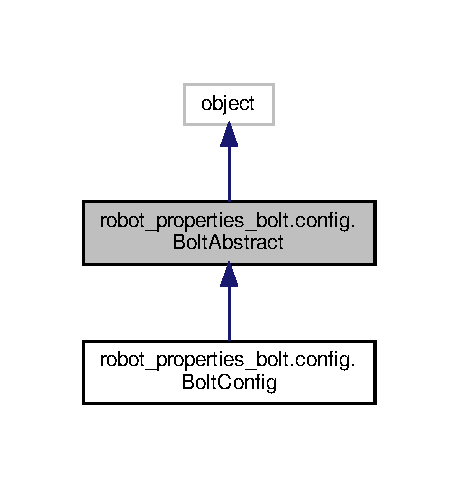
\includegraphics[width=220pt]{classrobot__properties__bolt_1_1config_1_1BoltAbstract__inherit__graph}
\end{center}
\end{figure}


Collaboration diagram for robot\+\_\+properties\+\_\+bolt.\+config.\+Bolt\+Abstract\+:
\nopagebreak
\begin{figure}[H]
\begin{center}
\leavevmode
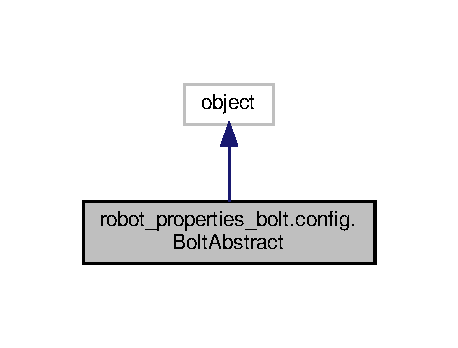
\includegraphics[width=220pt]{classrobot__properties__bolt_1_1config_1_1BoltAbstract__coll__graph}
\end{center}
\end{figure}
\subsection*{Public Member Functions}
\begin{DoxyCompactItemize}
\item 
\mbox{\Hypertarget{classrobot__properties__bolt_1_1config_1_1BoltAbstract_a7dc3456f295968793ca7cf0587a97454}\label{classrobot__properties__bolt_1_1config_1_1BoltAbstract_a7dc3456f295968793ca7cf0587a97454}} 
def {\bfseries build\+Robot\+Wrapper} (cls)
\item 
\mbox{\Hypertarget{classrobot__properties__bolt_1_1config_1_1BoltAbstract_aaab0127083f99286d766346af664bc5e}\label{classrobot__properties__bolt_1_1config_1_1BoltAbstract_aaab0127083f99286d766346af664bc5e}} 
def {\bfseries joint\+\_\+name\+\_\+in\+\_\+single\+\_\+string} (self)
\end{DoxyCompactItemize}
\subsection*{Static Public Attributes}
\begin{DoxyCompactItemize}
\item 
\mbox{\Hypertarget{classrobot__properties__bolt_1_1config_1_1BoltAbstract_acbf1c22583ad952bcc44da2a2ecd6a37}\label{classrobot__properties__bolt_1_1config_1_1BoltAbstract_acbf1c22583ad952bcc44da2a2ecd6a37}} 
float {\bfseries kp} = 5.\+0
\item 
\mbox{\Hypertarget{classrobot__properties__bolt_1_1config_1_1BoltAbstract_a0e28f7c221b04a4c1e1c17c70e36082a}\label{classrobot__properties__bolt_1_1config_1_1BoltAbstract_a0e28f7c221b04a4c1e1c17c70e36082a}} 
float {\bfseries kd} = 0.\+1
\item 
\mbox{\Hypertarget{classrobot__properties__bolt_1_1config_1_1BoltAbstract_aca4343ff9e5859dd648ce7a6d72ac9a2}\label{classrobot__properties__bolt_1_1config_1_1BoltAbstract_aca4343ff9e5859dd648ce7a6d72ac9a2}} 
float {\bfseries ki} = 0.\+0
\item 
\mbox{\Hypertarget{classrobot__properties__bolt_1_1config_1_1BoltAbstract_a4a989772e9a927e7e7bcaf8d0fc56eff}\label{classrobot__properties__bolt_1_1config_1_1BoltAbstract_a4a989772e9a927e7e7bcaf8d0fc56eff}} 
float {\bfseries motor\+\_\+torque\+\_\+constant} = 0.\+025
\item 
\mbox{\Hypertarget{classrobot__properties__bolt_1_1config_1_1BoltAbstract_a458bd418b9c7445a52c8949143aac53a}\label{classrobot__properties__bolt_1_1config_1_1BoltAbstract_a458bd418b9c7445a52c8949143aac53a}} 
float {\bfseries control\+\_\+period} = 0.\+001
\item 
\mbox{\Hypertarget{classrobot__properties__bolt_1_1config_1_1BoltAbstract_a7e4b05c34dff03c57b8993e3ba607b7d}\label{classrobot__properties__bolt_1_1config_1_1BoltAbstract_a7e4b05c34dff03c57b8993e3ba607b7d}} 
float {\bfseries dt} = control\+\_\+period
\item 
\mbox{\Hypertarget{classrobot__properties__bolt_1_1config_1_1BoltAbstract_affa85a628826e3f7cddeff5341f2c92e}\label{classrobot__properties__bolt_1_1config_1_1BoltAbstract_affa85a628826e3f7cddeff5341f2c92e}} 
int {\bfseries max\+\_\+current} = 2
\item 
\mbox{\Hypertarget{classrobot__properties__bolt_1_1config_1_1BoltAbstract_aef2224102582b76575515484857ba15b}\label{classrobot__properties__bolt_1_1config_1_1BoltAbstract_aef2224102582b76575515484857ba15b}} 
float {\bfseries max\+\_\+torque} = motor\+\_\+torque\+\_\+constant $\ast$ max\+\_\+current
\item 
\mbox{\Hypertarget{classrobot__properties__bolt_1_1config_1_1BoltAbstract_a34b90f440634b8761059d7bb6d1e781a}\label{classrobot__properties__bolt_1_1config_1_1BoltAbstract_a34b90f440634b8761059d7bb6d1e781a}} 
int {\bfseries max\+\_\+control} = max\+\_\+current
\item 
\mbox{\Hypertarget{classrobot__properties__bolt_1_1config_1_1BoltAbstract_a66654057aee624d4e9e8024e1f13a508}\label{classrobot__properties__bolt_1_1config_1_1BoltAbstract_a66654057aee624d4e9e8024e1f13a508}} 
float {\bfseries ctrl\+\_\+manager\+\_\+current\+\_\+to\+\_\+control\+\_\+gain} = 1.\+0
\item 
\mbox{\Hypertarget{classrobot__properties__bolt_1_1config_1_1BoltAbstract_a9db1e36360424c48157b8ec3aef70c6d}\label{classrobot__properties__bolt_1_1config_1_1BoltAbstract_a9db1e36360424c48157b8ec3aef70c6d}} 
{\bfseries max\+\_\+qref} = pi
\item 
\mbox{\Hypertarget{classrobot__properties__bolt_1_1config_1_1BoltAbstract_aee1c823623d5dbd60fff89fdc510650b}\label{classrobot__properties__bolt_1_1config_1_1BoltAbstract_aee1c823623d5dbd60fff89fdc510650b}} 
string {\bfseries base\+\_\+link\+\_\+name} = \textquotesingle{}base\+\_\+link\textquotesingle{}
\item 
\mbox{\Hypertarget{classrobot__properties__bolt_1_1config_1_1BoltAbstract_a21c485748b5e683b6e39c8b9f2ec83df}\label{classrobot__properties__bolt_1_1config_1_1BoltAbstract_a21c485748b5e683b6e39c8b9f2ec83df}} 
list {\bfseries end\+\_\+effector\+\_\+names} = \mbox{[}\textquotesingle{}F\+L\+\_\+\+A\+N\+K\+LE\textquotesingle{}, \textquotesingle{}F\+R\+\_\+\+A\+N\+K\+LE\textquotesingle{}\mbox{]}
\end{DoxyCompactItemize}


\subsection{Detailed Description}
Abstract class used for all Bolt robots. 



The documentation for this class was generated from the following file\+:\begin{DoxyCompactItemize}
\item 
python/robot\+\_\+properties\+\_\+bolt/\hyperlink{config_8py}{config.\+py}\end{DoxyCompactItemize}

\hypertarget{classrobot__properties__bolt_1_1config_1_1BoltConfig}{}\section{robot\+\_\+properties\+\_\+bolt.\+config.\+Bolt\+Config Class Reference}
\label{classrobot__properties__bolt_1_1config_1_1BoltConfig}\index{robot\+\_\+properties\+\_\+bolt.\+config.\+Bolt\+Config@{robot\+\_\+properties\+\_\+bolt.\+config.\+Bolt\+Config}}


Inheritance diagram for robot\+\_\+properties\+\_\+bolt.\+config.\+Bolt\+Config\+:
\nopagebreak
\begin{figure}[H]
\begin{center}
\leavevmode
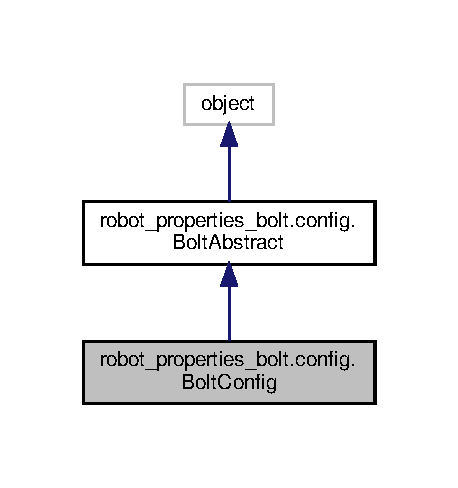
\includegraphics[width=220pt]{classrobot__properties__bolt_1_1config_1_1BoltConfig__inherit__graph}
\end{center}
\end{figure}


Collaboration diagram for robot\+\_\+properties\+\_\+bolt.\+config.\+Bolt\+Config\+:
\nopagebreak
\begin{figure}[H]
\begin{center}
\leavevmode
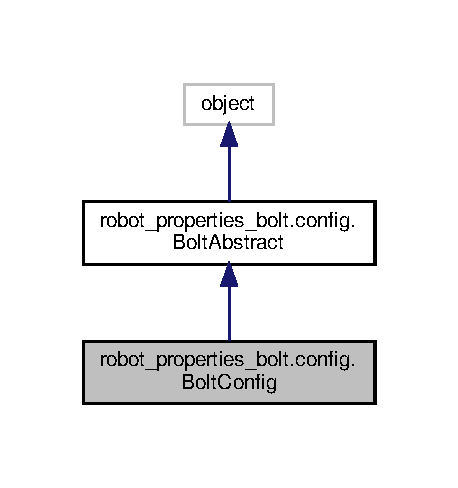
\includegraphics[width=220pt]{classrobot__properties__bolt_1_1config_1_1BoltConfig__coll__graph}
\end{center}
\end{figure}
\subsection*{Static Public Attributes}
\begin{DoxyCompactItemize}
\item 
\mbox{\Hypertarget{classrobot__properties__bolt_1_1config_1_1BoltConfig_a2ae10e99a7cba2220217c56d1a4d574f}\label{classrobot__properties__bolt_1_1config_1_1BoltConfig_a2ae10e99a7cba2220217c56d1a4d574f}} 
string {\bfseries robot\+\_\+family} = \char`\"{}bolt\char`\"{}
\item 
\mbox{\Hypertarget{classrobot__properties__bolt_1_1config_1_1BoltConfig_ad95290beb57b4a2b73ae771cd48775a8}\label{classrobot__properties__bolt_1_1config_1_1BoltConfig_ad95290beb57b4a2b73ae771cd48775a8}} 
string {\bfseries robot\+\_\+name} = \char`\"{}bolt\char`\"{}
\item 
tuple {\bfseries urdf\+\_\+path}
\item 
list {\bfseries meshes\+\_\+path}
\item 
tuple {\bfseries yaml\+\_\+path}
\item 
\mbox{\Hypertarget{classrobot__properties__bolt_1_1config_1_1BoltConfig_a3845b64e9c77be3a4c86c4759a524421}\label{classrobot__properties__bolt_1_1config_1_1BoltConfig_a3845b64e9c77be3a4c86c4759a524421}} 
float {\bfseries motor\+\_\+inertia} = 0.\+0000045
\item 
\mbox{\Hypertarget{classrobot__properties__bolt_1_1config_1_1BoltConfig_ac4ecaff049f5b2100d4f7a00ce636acd}\label{classrobot__properties__bolt_1_1config_1_1BoltConfig_ac4ecaff049f5b2100d4f7a00ce636acd}} 
int {\bfseries motor\+\_\+gear\+\_\+ration} = 9.
\item 
{\bfseries robot\+\_\+model}
\item 
\mbox{\Hypertarget{classrobot__properties__bolt_1_1config_1_1BoltConfig_af1f4a09c638014176ef3d2070641e3c0}\label{classrobot__properties__bolt_1_1config_1_1BoltConfig_af1f4a09c638014176ef3d2070641e3c0}} 
{\bfseries mass} = np.\+sum(\mbox{[}i.\+mass for i in robot\+\_\+model.\+inertias\mbox{]})
\item 
\mbox{\Hypertarget{classrobot__properties__bolt_1_1config_1_1BoltConfig_ac17e14abb668429480eb737ab8809de4}\label{classrobot__properties__bolt_1_1config_1_1BoltConfig_ac17e14abb668429480eb737ab8809de4}} 
{\bfseries base\+\_\+name} = robot\+\_\+model.\+frames\mbox{[}2\mbox{]}.name
\item 
\mbox{\Hypertarget{classrobot__properties__bolt_1_1config_1_1BoltConfig_af7b7472e47666cc878722d3723be8842}\label{classrobot__properties__bolt_1_1config_1_1BoltConfig_af7b7472e47666cc878722d3723be8842}} 
int {\bfseries nb\+\_\+joints} = robot\+\_\+model.\+nv -\/ 6
\item 
\mbox{\Hypertarget{classrobot__properties__bolt_1_1config_1_1BoltConfig_aa87bcf63201b8b78e6dcfbccf07780f5}\label{classrobot__properties__bolt_1_1config_1_1BoltConfig_aa87bcf63201b8b78e6dcfbccf07780f5}} 
list {\bfseries joint\+\_\+names} = \mbox{[}\textquotesingle{}F\+L\+\_\+\+H\+AA\textquotesingle{}, \textquotesingle{}F\+L\+\_\+\+H\+FE\textquotesingle{}, \textquotesingle{}F\+L\+\_\+\+K\+FE\textquotesingle{}, \textquotesingle{}F\+R\+\_\+\+H\+AA\textquotesingle{}, \textquotesingle{}F\+R\+\_\+\+H\+FE\textquotesingle{}, \textquotesingle{}F\+R\+\_\+\+K\+FE\textquotesingle{}\mbox{]}
\item 
\mbox{\Hypertarget{classrobot__properties__bolt_1_1config_1_1BoltConfig_aeb232d8cf65792a9b0d32f2ab997e43e}\label{classrobot__properties__bolt_1_1config_1_1BoltConfig_aeb232d8cf65792a9b0d32f2ab997e43e}} 
{\bfseries urdf\+\_\+to\+\_\+dgm} = tuple(range(6))
\item 
\mbox{\Hypertarget{classrobot__properties__bolt_1_1config_1_1BoltConfig_a597a95163a443768ee1c800e18487673}\label{classrobot__properties__bolt_1_1config_1_1BoltConfig_a597a95163a443768ee1c800e18487673}} 
dictionary {\bfseries map\+\_\+joint\+\_\+name\+\_\+to\+\_\+id} = \{\}
\item 
\mbox{\Hypertarget{classrobot__properties__bolt_1_1config_1_1BoltConfig_a44b06cd0b41a6d0458a55d152248afd7}\label{classrobot__properties__bolt_1_1config_1_1BoltConfig_a44b06cd0b41a6d0458a55d152248afd7}} 
dictionary {\bfseries map\+\_\+joint\+\_\+limits} = \{\}
\item 
{\bfseries initial\+\_\+configuration}
\item 
\mbox{\Hypertarget{classrobot__properties__bolt_1_1config_1_1BoltConfig_a812b933772fdaa3af006db16906ecd67}\label{classrobot__properties__bolt_1_1config_1_1BoltConfig_a812b933772fdaa3af006db16906ecd67}} 
tuple {\bfseries initial\+\_\+velocity} = (6 + 6)$\ast$\mbox{[}0, \mbox{]}
\item 
\mbox{\Hypertarget{classrobot__properties__bolt_1_1config_1_1BoltConfig_a3ca925730077785d60c002e54007a82f}\label{classrobot__properties__bolt_1_1config_1_1BoltConfig_a3ca925730077785d60c002e54007a82f}} 
{\bfseries q0} = np.\+zeros(robot\+\_\+model.\+nq)
\item 
\mbox{\Hypertarget{classrobot__properties__bolt_1_1config_1_1BoltConfig_a8a30825588f84a0d61781b0a0667a99c}\label{classrobot__properties__bolt_1_1config_1_1BoltConfig_a8a30825588f84a0d61781b0a0667a99c}} 
{\bfseries v0} = np.\+zeros(robot\+\_\+model.\+nv)
\item 
\mbox{\Hypertarget{classrobot__properties__bolt_1_1config_1_1BoltConfig_a47c3a0f37835ca3d09c2aefffbcc2255}\label{classrobot__properties__bolt_1_1config_1_1BoltConfig_a47c3a0f37835ca3d09c2aefffbcc2255}} 
{\bfseries a0} = np.\+zeros(robot\+\_\+model.\+nv)
\end{DoxyCompactItemize}
\subsection*{Additional Inherited Members}


\subsection{Member Data Documentation}
\mbox{\Hypertarget{classrobot__properties__bolt_1_1config_1_1BoltConfig_af8743a94646c654f4743780f5b6069d0}\label{classrobot__properties__bolt_1_1config_1_1BoltConfig_af8743a94646c654f4743780f5b6069d0}} 
\index{robot\+\_\+properties\+\_\+bolt\+::config\+::\+Bolt\+Config@{robot\+\_\+properties\+\_\+bolt\+::config\+::\+Bolt\+Config}!initial\+\_\+configuration@{initial\+\_\+configuration}}
\index{initial\+\_\+configuration@{initial\+\_\+configuration}!robot\+\_\+properties\+\_\+bolt\+::config\+::\+Bolt\+Config@{robot\+\_\+properties\+\_\+bolt\+::config\+::\+Bolt\+Config}}
\subsubsection{\texorpdfstring{initial\+\_\+configuration}{initial\_configuration}}
{\footnotesize\ttfamily robot\+\_\+properties\+\_\+bolt.\+config.\+Bolt\+Config.\+initial\+\_\+configuration\hspace{0.3cm}{\ttfamily [static]}}

{\bfseries Initial value\+:}
\begin{DoxyCode}
=  np.array(
        [0., 0., 0.26487417, 0., 0., 0., 1.,
         -0.35, -0.78539816, 1.57079633, 0.35, -0.78539816, 1.57079633])
\end{DoxyCode}
\mbox{\Hypertarget{classrobot__properties__bolt_1_1config_1_1BoltConfig_ace1b01ce0da5692a5bbfb8722009948a}\label{classrobot__properties__bolt_1_1config_1_1BoltConfig_ace1b01ce0da5692a5bbfb8722009948a}} 
\index{robot\+\_\+properties\+\_\+bolt\+::config\+::\+Bolt\+Config@{robot\+\_\+properties\+\_\+bolt\+::config\+::\+Bolt\+Config}!meshes\+\_\+path@{meshes\+\_\+path}}
\index{meshes\+\_\+path@{meshes\+\_\+path}!robot\+\_\+properties\+\_\+bolt\+::config\+::\+Bolt\+Config@{robot\+\_\+properties\+\_\+bolt\+::config\+::\+Bolt\+Config}}
\subsubsection{\texorpdfstring{meshes\+\_\+path}{meshes\_path}}
{\footnotesize\ttfamily list robot\+\_\+properties\+\_\+bolt.\+config.\+Bolt\+Config.\+meshes\+\_\+path\hspace{0.3cm}{\ttfamily [static]}}

{\bfseries Initial value\+:}
\begin{DoxyCode}
=  [
        dirname(rospkg.RosPack().get\_path(\textcolor{stringliteral}{"robot\_properties\_"} + robot\_family))
    ]
\end{DoxyCode}
\mbox{\Hypertarget{classrobot__properties__bolt_1_1config_1_1BoltConfig_aa4a7242bb7ba6bab2b49ad1abad3c285}\label{classrobot__properties__bolt_1_1config_1_1BoltConfig_aa4a7242bb7ba6bab2b49ad1abad3c285}} 
\index{robot\+\_\+properties\+\_\+bolt\+::config\+::\+Bolt\+Config@{robot\+\_\+properties\+\_\+bolt\+::config\+::\+Bolt\+Config}!robot\+\_\+model@{robot\+\_\+model}}
\index{robot\+\_\+model@{robot\+\_\+model}!robot\+\_\+properties\+\_\+bolt\+::config\+::\+Bolt\+Config@{robot\+\_\+properties\+\_\+bolt\+::config\+::\+Bolt\+Config}}
\subsubsection{\texorpdfstring{robot\+\_\+model}{robot\_model}}
{\footnotesize\ttfamily robot\+\_\+properties\+\_\+bolt.\+config.\+Bolt\+Config.\+robot\+\_\+model\hspace{0.3cm}{\ttfamily [static]}}

{\bfseries Initial value\+:}
\begin{DoxyCode}
=  se3.buildModelFromUrdf(urdf\_path,
                                         se3.JointModelFreeFlyer())
\end{DoxyCode}
\mbox{\Hypertarget{classrobot__properties__bolt_1_1config_1_1BoltConfig_a5872ce325d36cca7b5c8ef9555e6ed66}\label{classrobot__properties__bolt_1_1config_1_1BoltConfig_a5872ce325d36cca7b5c8ef9555e6ed66}} 
\index{robot\+\_\+properties\+\_\+bolt\+::config\+::\+Bolt\+Config@{robot\+\_\+properties\+\_\+bolt\+::config\+::\+Bolt\+Config}!urdf\+\_\+path@{urdf\+\_\+path}}
\index{urdf\+\_\+path@{urdf\+\_\+path}!robot\+\_\+properties\+\_\+bolt\+::config\+::\+Bolt\+Config@{robot\+\_\+properties\+\_\+bolt\+::config\+::\+Bolt\+Config}}
\subsubsection{\texorpdfstring{urdf\+\_\+path}{urdf\_path}}
{\footnotesize\ttfamily tuple robot\+\_\+properties\+\_\+bolt.\+config.\+Bolt\+Config.\+urdf\+\_\+path\hspace{0.3cm}{\ttfamily [static]}}

{\bfseries Initial value\+:}
\begin{DoxyCode}
=  (
        join(rospkg.RosPack().get\_path(\textcolor{stringliteral}{"robot\_properties\_"} + robot\_family),
             \textcolor{stringliteral}{"urdf"},
             robot\_name + \textcolor{stringliteral}{".urdf"})
    )
\end{DoxyCode}
\mbox{\Hypertarget{classrobot__properties__bolt_1_1config_1_1BoltConfig_a814bb92fd8297c1ab7621e0d4adf5471}\label{classrobot__properties__bolt_1_1config_1_1BoltConfig_a814bb92fd8297c1ab7621e0d4adf5471}} 
\index{robot\+\_\+properties\+\_\+bolt\+::config\+::\+Bolt\+Config@{robot\+\_\+properties\+\_\+bolt\+::config\+::\+Bolt\+Config}!yaml\+\_\+path@{yaml\+\_\+path}}
\index{yaml\+\_\+path@{yaml\+\_\+path}!robot\+\_\+properties\+\_\+bolt\+::config\+::\+Bolt\+Config@{robot\+\_\+properties\+\_\+bolt\+::config\+::\+Bolt\+Config}}
\subsubsection{\texorpdfstring{yaml\+\_\+path}{yaml\_path}}
{\footnotesize\ttfamily tuple robot\+\_\+properties\+\_\+bolt.\+config.\+Bolt\+Config.\+yaml\+\_\+path\hspace{0.3cm}{\ttfamily [static]}}

{\bfseries Initial value\+:}
\begin{DoxyCode}
=  (
        join(rospkg.RosPack().get\_path(\textcolor{stringliteral}{"robot\_properties\_"} + robot\_family),
             \textcolor{stringliteral}{"config"},
             \textcolor{stringliteral}{"dgm\_parameters\_bolt.yaml"})
    )
\end{DoxyCode}


The documentation for this class was generated from the following file\+:\begin{DoxyCompactItemize}
\item 
python/robot\+\_\+properties\+\_\+bolt/\hyperlink{config_8py}{config.\+py}\end{DoxyCompactItemize}

\hypertarget{classrobot__properties__bolt_1_1bolt__wrapper_1_1BoltRobot}{}\section{robot\+\_\+properties\+\_\+bolt.\+bolt\+\_\+wrapper.\+Bolt\+Robot Class Reference}
\label{classrobot__properties__bolt_1_1bolt__wrapper_1_1BoltRobot}\index{robot\+\_\+properties\+\_\+bolt.\+bolt\+\_\+wrapper.\+Bolt\+Robot@{robot\+\_\+properties\+\_\+bolt.\+bolt\+\_\+wrapper.\+Bolt\+Robot}}


Inheritance diagram for robot\+\_\+properties\+\_\+bolt.\+bolt\+\_\+wrapper.\+Bolt\+Robot\+:
\nopagebreak
\begin{figure}[H]
\begin{center}
\leavevmode
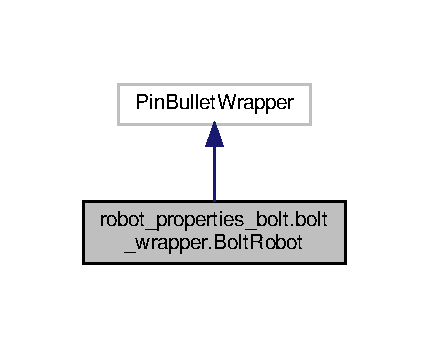
\includegraphics[width=206pt]{classrobot__properties__bolt_1_1bolt__wrapper_1_1BoltRobot__inherit__graph}
\end{center}
\end{figure}


Collaboration diagram for robot\+\_\+properties\+\_\+bolt.\+bolt\+\_\+wrapper.\+Bolt\+Robot\+:
\nopagebreak
\begin{figure}[H]
\begin{center}
\leavevmode
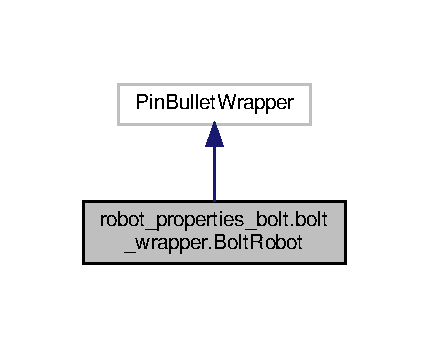
\includegraphics[width=206pt]{classrobot__properties__bolt_1_1bolt__wrapper_1_1BoltRobot__coll__graph}
\end{center}
\end{figure}
\subsection*{Public Member Functions}
\begin{DoxyCompactItemize}
\item 
\mbox{\Hypertarget{classrobot__properties__bolt_1_1bolt__wrapper_1_1BoltRobot_acc76618b714d456c7765a9b28dbcf26b}\label{classrobot__properties__bolt_1_1bolt__wrapper_1_1BoltRobot_acc76618b714d456c7765a9b28dbcf26b}} 
def {\bfseries \+\_\+\+\_\+init\+\_\+\+\_\+} (self, physics\+Client=None)
\item 
\mbox{\Hypertarget{classrobot__properties__bolt_1_1bolt__wrapper_1_1BoltRobot_ae17d151dc47a026007eb4c6764a1e1e7}\label{classrobot__properties__bolt_1_1bolt__wrapper_1_1BoltRobot_ae17d151dc47a026007eb4c6764a1e1e7}} 
def {\bfseries forward\+\_\+robot} (self, q=None, dq=None)
\end{DoxyCompactItemize}
\subsection*{Static Public Member Functions}
\begin{DoxyCompactItemize}
\item 
\mbox{\Hypertarget{classrobot__properties__bolt_1_1bolt__wrapper_1_1BoltRobot_a43802302483bc1987831b9b607892b2a}\label{classrobot__properties__bolt_1_1bolt__wrapper_1_1BoltRobot_a43802302483bc1987831b9b607892b2a}} 
def {\bfseries init\+Physics\+Client} ()
\end{DoxyCompactItemize}
\subsection*{Public Attributes}
\begin{DoxyCompactItemize}
\item 
\mbox{\Hypertarget{classrobot__properties__bolt_1_1bolt__wrapper_1_1BoltRobot_ae9ef071c3c94d387b28dd7195868cf2b}\label{classrobot__properties__bolt_1_1bolt__wrapper_1_1BoltRobot_ae9ef071c3c94d387b28dd7195868cf2b}} 
{\bfseries physics\+Client}
\item 
\mbox{\Hypertarget{classrobot__properties__bolt_1_1bolt__wrapper_1_1BoltRobot_aeeed18e70d5bad25ed47f179ce668e4b}\label{classrobot__properties__bolt_1_1bolt__wrapper_1_1BoltRobot_aeeed18e70d5bad25ed47f179ce668e4b}} 
{\bfseries plane\+Id}
\item 
\mbox{\Hypertarget{classrobot__properties__bolt_1_1bolt__wrapper_1_1BoltRobot_a3db6e1e7138a09310827f8d25fe54331}\label{classrobot__properties__bolt_1_1bolt__wrapper_1_1BoltRobot_a3db6e1e7138a09310827f8d25fe54331}} 
{\bfseries urdf\+\_\+path}
\item 
\mbox{\Hypertarget{classrobot__properties__bolt_1_1bolt__wrapper_1_1BoltRobot_a02d9fcdb5e81e374d2c91c27b884b484}\label{classrobot__properties__bolt_1_1bolt__wrapper_1_1BoltRobot_a02d9fcdb5e81e374d2c91c27b884b484}} 
{\bfseries robot\+Id}
\item 
\mbox{\Hypertarget{classrobot__properties__bolt_1_1bolt__wrapper_1_1BoltRobot_a097d46d9389c25aae160a5d595619d9a}\label{classrobot__properties__bolt_1_1bolt__wrapper_1_1BoltRobot_a097d46d9389c25aae160a5d595619d9a}} 
{\bfseries pin\+\_\+robot}
\item 
\mbox{\Hypertarget{classrobot__properties__bolt_1_1bolt__wrapper_1_1BoltRobot_abe62f94e6d7cbb48294153e97b55a59e}\label{classrobot__properties__bolt_1_1bolt__wrapper_1_1BoltRobot_abe62f94e6d7cbb48294153e97b55a59e}} 
{\bfseries base\+\_\+link\+\_\+name}
\item 
\mbox{\Hypertarget{classrobot__properties__bolt_1_1bolt__wrapper_1_1BoltRobot_a0e8e5c5325b4bcae1167c09ee47dc74f}\label{classrobot__properties__bolt_1_1bolt__wrapper_1_1BoltRobot_a0e8e5c5325b4bcae1167c09ee47dc74f}} 
{\bfseries joint\+\_\+names}
\item 
\mbox{\Hypertarget{classrobot__properties__bolt_1_1bolt__wrapper_1_1BoltRobot_ae09860f85eab00ed00dd49781a652be3}\label{classrobot__properties__bolt_1_1bolt__wrapper_1_1BoltRobot_ae09860f85eab00ed00dd49781a652be3}} 
{\bfseries end\+\_\+effector\+\_\+names}
\end{DoxyCompactItemize}


The documentation for this class was generated from the following file\+:\begin{DoxyCompactItemize}
\item 
python/robot\+\_\+properties\+\_\+bolt/bolt\+\_\+wrapper.\+py\end{DoxyCompactItemize}

\chapter{File Documentation}
\hypertarget{display__bolt_8py}{}\section{demos/display\+\_\+bolt.py File Reference}
\label{display__bolt_8py}\index{demos/display\+\_\+bolt.\+py@{demos/display\+\_\+bolt.\+py}}
\subsection*{Namespaces}
\begin{DoxyCompactItemize}
\item 
 \hyperlink{namespaceBasic}{Basic}
\begin{DoxyCompactList}\small\item\em loading and visualization for the Bolt robot using gepetto viewer. \end{DoxyCompactList}\end{DoxyCompactItemize}
\subsection*{Variables}
\begin{DoxyCompactItemize}
\item 
\mbox{\Hypertarget{display__bolt_8py_a189e4f90dfb67881c750a27438e99951}\label{display__bolt_8py_a189e4f90dfb67881c750a27438e99951}} 
{\bfseries display\+\_\+bolt.\+robot} = Bolt\+Config.\+build\+Robot\+Wrapper()
\item 
\mbox{\Hypertarget{display__bolt_8py_a2aa0d405f2e8ac4c5becc04f58c81ce1}\label{display__bolt_8py_a2aa0d405f2e8ac4c5becc04f58c81ce1}} 
{\bfseries display\+\_\+bolt.\+load\+Model}
\item 
\mbox{\Hypertarget{display__bolt_8py_a11f488d2842bf0818b26e0fe4c2c99c4}\label{display__bolt_8py_a11f488d2842bf0818b26e0fe4c2c99c4}} 
{\bfseries display\+\_\+bolt.\+q} = Bolt\+Config.\+initial\+\_\+configuration
\end{DoxyCompactItemize}


\subsection{Detailed Description}
\begin{DoxyCopyright}{Copyright}
Copyright (c) 2020, New York University and Max Planck Gesellschaft, License B\+S\+D-\/3-\/\+Clause 
\end{DoxyCopyright}

\hypertarget{____init_____8py}{}\section{python/robot\+\_\+properties\+\_\+bolt/\+\_\+\+\_\+init\+\_\+\+\_\+.py File Reference}
\label{____init_____8py}\index{python/robot\+\_\+properties\+\_\+bolt/\+\_\+\+\_\+init\+\_\+\+\_\+.\+py@{python/robot\+\_\+properties\+\_\+bolt/\+\_\+\+\_\+init\+\_\+\+\_\+.\+py}}
\subsection*{Namespaces}
\begin{DoxyCompactItemize}
\item 
 \hyperlink{namespaceci__example__python}{ci\+\_\+example\+\_\+python}
\begin{DoxyCompactList}\small\item\em Contains an example of a python package. \end{DoxyCompactList}\end{DoxyCompactItemize}
\subsection*{Variables}
\begin{DoxyCompactItemize}
\item 
\mbox{\Hypertarget{____init_____8py_a217db87422e5ebde4fa29c582c3291ba}\label{____init_____8py_a217db87422e5ebde4fa29c582c3291ba}} 
string {\bfseries robot\+\_\+properties\+\_\+bolt.\+\_\+\+\_\+copyright\+\_\+\+\_\+} = \char`\"{}Copyright (c) 2020, New York University and Max Planck Gesellschaft.\char`\"{}
\item 
\mbox{\Hypertarget{____init_____8py_a0f340f6aee0dd088bfcd10fc9fcf943c}\label{____init_____8py_a0f340f6aee0dd088bfcd10fc9fcf943c}} 
string {\bfseries robot\+\_\+properties\+\_\+bolt.\+\_\+\+\_\+license\+\_\+\+\_\+} = \char`\"{}B\+SD 3-\/Clause\char`\"{}
\item 
\mbox{\Hypertarget{____init_____8py_a7904c4b5246d346d651124bfaef8c722}\label{____init_____8py_a7904c4b5246d346d651124bfaef8c722}} 
string {\bfseries robot\+\_\+properties\+\_\+bolt.\+\_\+\+\_\+version\+\_\+\+\_\+} = \char`\"{}0.\+0.\+0\char`\"{}
\item 
\mbox{\Hypertarget{____init_____8py_ad4dc162f84ed9434980c2f816c676e86}\label{____init_____8py_ad4dc162f84ed9434980c2f816c676e86}} 
string {\bfseries robot\+\_\+properties\+\_\+bolt.\+\_\+\+\_\+status\+\_\+\+\_\+} = \char`\"{}Done\char`\"{}
\end{DoxyCompactItemize}

\hypertarget{config_8py}{}\section{python/robot\+\_\+properties\+\_\+bolt/config.py File Reference}
\label{config_8py}\index{python/robot\+\_\+properties\+\_\+bolt/config.\+py@{python/robot\+\_\+properties\+\_\+bolt/config.\+py}}


This module includes configuration for the Bolt.  


\subsection*{Classes}
\begin{DoxyCompactItemize}
\item 
class \hyperlink{classrobot__properties__bolt_1_1config_1_1BoltAbstract}{robot\+\_\+properties\+\_\+bolt.\+config.\+Bolt\+Abstract}
\begin{DoxyCompactList}\small\item\em Abstract class used for all Bolt robots. \end{DoxyCompactList}\item 
class \hyperlink{classrobot__properties__bolt_1_1config_1_1BoltConfig}{robot\+\_\+properties\+\_\+bolt.\+config.\+Bolt\+Config}
\end{DoxyCompactItemize}


\subsection{Detailed Description}
This module includes configuration for the Bolt. 

\begin{DoxyCopyright}{Copyright}
Copyright (c) 2020, New York University and Max Planck Gesellschaft, License B\+S\+D-\/3-\/\+Clause 
\end{DoxyCopyright}

\hypertarget{gepetto__gui__loader_8py}{}\section{python/robot\+\_\+properties\+\_\+bolt/gepetto\+\_\+gui\+\_\+loader.py File Reference}
\label{gepetto__gui__loader_8py}\index{python/robot\+\_\+properties\+\_\+bolt/gepetto\+\_\+gui\+\_\+loader.\+py@{python/robot\+\_\+properties\+\_\+bolt/gepetto\+\_\+gui\+\_\+loader.\+py}}
\subsection*{Namespaces}
\begin{DoxyCompactItemize}
\item 
 \hyperlink{namespacerobot__properties__bolt_1_1gepetto__gui__loader}{robot\+\_\+properties\+\_\+bolt.\+gepetto\+\_\+gui\+\_\+loader}
\begin{DoxyCompactList}\small\item\em This module shows Bolt in gepetto\+\_\+gui. \end{DoxyCompactList}\end{DoxyCompactItemize}
\subsection*{Functions}
\begin{DoxyCompactItemize}
\item 
\mbox{\Hypertarget{namespacerobot__properties__bolt_1_1gepetto__gui__loader_a5d8d39b75280e377bb5b230a0283b6c7}\label{namespacerobot__properties__bolt_1_1gepetto__gui__loader_a5d8d39b75280e377bb5b230a0283b6c7}} 
def \hyperlink{namespacerobot__properties__bolt_1_1gepetto__gui__loader_a5d8d39b75280e377bb5b230a0283b6c7}{robot\+\_\+properties\+\_\+bolt.\+gepetto\+\_\+gui\+\_\+loader.\+create\+\_\+scene} ()
\begin{DoxyCompactList}\small\item\em Just create a scene for the bolt to be in. \end{DoxyCompactList}\item 
\mbox{\Hypertarget{namespacerobot__properties__bolt_1_1gepetto__gui__loader_acce27d25ffff793eda1befea8fb7a7de}\label{namespacerobot__properties__bolt_1_1gepetto__gui__loader_acce27d25ffff793eda1befea8fb7a7de}} 
def \hyperlink{namespacerobot__properties__bolt_1_1gepetto__gui__loader_acce27d25ffff793eda1befea8fb7a7de}{robot\+\_\+properties\+\_\+bolt.\+gepetto\+\_\+gui\+\_\+loader.\+load\+\_\+bolt\+\_\+in\+\_\+gepetto\+\_\+gui} (gepetto\+\_\+scene, robot\+\_\+name)
\begin{DoxyCompactList}\small\item\em Load the bolt meshes in the scene. \end{DoxyCompactList}\item 
\mbox{\Hypertarget{namespacerobot__properties__bolt_1_1gepetto__gui__loader_a3d01306696eb724d0e3489865ac0c376}\label{namespacerobot__properties__bolt_1_1gepetto__gui__loader_a3d01306696eb724d0e3489865ac0c376}} 
def {\bfseries robot\+\_\+properties\+\_\+bolt.\+gepetto\+\_\+gui\+\_\+loader.\+display\+\_\+bolt\+\_\+in\+\_\+gepetto\+\_\+gui} (launch\+\_\+gepetto\+\_\+gui\+\_\+exec=False)
\end{DoxyCompactItemize}


\subsection{Detailed Description}
\begin{DoxyCopyright}{Copyright}
Copyright (c) 2020, New York University and Max Planck Gesellschaft, License B\+S\+D-\/3-\/\+Clause 
\end{DoxyCopyright}

\hypertarget{pd_8py}{}\section{python/robot\+\_\+properties\+\_\+bolt/pd.py File Reference}
\label{pd_8py}\index{python/robot\+\_\+properties\+\_\+bolt/pd.\+py@{python/robot\+\_\+properties\+\_\+bolt/pd.\+py}}
\subsection*{Namespaces}
\begin{DoxyCompactItemize}
\item 
 \hyperlink{namespacerobot__properties__bolt_1_1pd}{robot\+\_\+properties\+\_\+bolt.\+pd}
\begin{DoxyCompactList}\small\item\em This module reads planner data from files and runs a PD controller. \end{DoxyCompactList}\end{DoxyCompactItemize}
\subsection*{Functions}
\begin{DoxyCompactItemize}
\item 
\mbox{\Hypertarget{namespacerobot__properties__bolt_1_1pd_aefad3d3447a097bbda79da022146dc01}\label{namespacerobot__properties__bolt_1_1pd_aefad3d3447a097bbda79da022146dc01}} 
def {\bfseries robot\+\_\+properties\+\_\+bolt.\+pd.\+plot} ()
\end{DoxyCompactItemize}
\subsection*{Variables}
\begin{DoxyCompactItemize}
\item 
\mbox{\Hypertarget{namespacerobot__properties__bolt_1_1pd_a4ea1ee8c05aad280197204fb29e4e503}\label{namespacerobot__properties__bolt_1_1pd_a4ea1ee8c05aad280197204fb29e4e503}} 
{\bfseries robot\+\_\+properties\+\_\+bolt.\+pd.\+robot} = Bolt\+Robot()
\item 
\mbox{\Hypertarget{namespacerobot__properties__bolt_1_1pd_aaa85f193a577d2844e0ef55ff88a3b92}\label{namespacerobot__properties__bolt_1_1pd_aaa85f193a577d2844e0ef55ff88a3b92}} 
{\bfseries robot\+\_\+properties\+\_\+bolt.\+pd.\+torque} = np.\+loadtxt(\char`\"{}Torque.\+txt\char`\"{})
\item 
\mbox{\Hypertarget{namespacerobot__properties__bolt_1_1pd_a9659711d6dd60b9130da2f187ad45ce1}\label{namespacerobot__properties__bolt_1_1pd_a9659711d6dd60b9130da2f187ad45ce1}} 
{\bfseries robot\+\_\+properties\+\_\+bolt.\+pd.\+pos} = np.\+loadtxt(\char`\"{}Position.\+txt\char`\"{})
\item 
\mbox{\Hypertarget{namespacerobot__properties__bolt_1_1pd_aec9f899bd4d65c3af623ad8ba7766921}\label{namespacerobot__properties__bolt_1_1pd_aec9f899bd4d65c3af623ad8ba7766921}} 
{\bfseries robot\+\_\+properties\+\_\+bolt.\+pd.\+vel} = np.\+loadtxt(\char`\"{}Velocity.\+txt\char`\"{})
\item 
\mbox{\Hypertarget{namespacerobot__properties__bolt_1_1pd_a0aaa7a1517bdb4c50d64270c7793e25f}\label{namespacerobot__properties__bolt_1_1pd_a0aaa7a1517bdb4c50d64270c7793e25f}} 
{\bfseries robot\+\_\+properties\+\_\+bolt.\+pd.\+q0} = Bolt\+Config.\+initial\+\_\+configuration
\item 
\mbox{\Hypertarget{namespacerobot__properties__bolt_1_1pd_a8c20dabb913f3b7dd3ac129f20d087ea}\label{namespacerobot__properties__bolt_1_1pd_a8c20dabb913f3b7dd3ac129f20d087ea}} 
{\bfseries robot\+\_\+properties\+\_\+bolt.\+pd.\+dq0} = Bolt\+Config.\+initial\+\_\+velocity
\item 
\mbox{\Hypertarget{namespacerobot__properties__bolt_1_1pd_ac45beac2298c90f363b3a6d41d1f0a7d}\label{namespacerobot__properties__bolt_1_1pd_ac45beac2298c90f363b3a6d41d1f0a7d}} 
int {\bfseries robot\+\_\+properties\+\_\+bolt.\+pd.\+kp} = 20
\item 
\mbox{\Hypertarget{namespacerobot__properties__bolt_1_1pd_ac1f10d4b84bc9dea26f7c4cd8e72e248}\label{namespacerobot__properties__bolt_1_1pd_ac1f10d4b84bc9dea26f7c4cd8e72e248}} 
float {\bfseries robot\+\_\+properties\+\_\+bolt.\+pd.\+kd} = 0.\+1
\item 
\mbox{\Hypertarget{namespacerobot__properties__bolt_1_1pd_a611603e2281532f181f08e35c72f8458}\label{namespacerobot__properties__bolt_1_1pd_a611603e2281532f181f08e35c72f8458}} 
list {\bfseries robot\+\_\+properties\+\_\+bolt.\+pd.\+pos\+History} = \mbox{[}$\,$\mbox{]}
\item 
\mbox{\Hypertarget{namespacerobot__properties__bolt_1_1pd_a9a39a51b2f763e8a21ef887e9e3d9798}\label{namespacerobot__properties__bolt_1_1pd_a9a39a51b2f763e8a21ef887e9e3d9798}} 
{\bfseries robot\+\_\+properties\+\_\+bolt.\+pd.\+delta\+Pos} = pos\mbox{[}i\mbox{]} -\/ np.\+squeeze(np.\+asarray(robot.\+get\+\_\+state()\mbox{[}0\mbox{]}\mbox{[}7\+:\mbox{]}))
\item 
\mbox{\Hypertarget{namespacerobot__properties__bolt_1_1pd_aba4eaf4c107132793a0b485aefaaafeb}\label{namespacerobot__properties__bolt_1_1pd_aba4eaf4c107132793a0b485aefaaafeb}} 
{\bfseries robot\+\_\+properties\+\_\+bolt.\+pd.\+delta\+Vel} = vel\mbox{[}i\mbox{]} -\/ np.\+squeeze(np.\+asarray(robot.\+get\+\_\+state()\mbox{[}1\mbox{]}\mbox{[}6\+:\mbox{]}))
\item 
\mbox{\Hypertarget{namespacerobot__properties__bolt_1_1pd_a34cb69b502b8932afd00a74d722f6f35}\label{namespacerobot__properties__bolt_1_1pd_a34cb69b502b8932afd00a74d722f6f35}} 
{\bfseries robot\+\_\+properties\+\_\+bolt.\+pd.\+q}
\item 
\mbox{\Hypertarget{namespacerobot__properties__bolt_1_1pd_a0a1e0aab2ba1ec88672f657be05c1ae5}\label{namespacerobot__properties__bolt_1_1pd_a0a1e0aab2ba1ec88672f657be05c1ae5}} 
{\bfseries robot\+\_\+properties\+\_\+bolt.\+pd.\+dq}
\item 
\mbox{\Hypertarget{namespacerobot__properties__bolt_1_1pd_aa6415397e803d7de4f890a0a81c65485}\label{namespacerobot__properties__bolt_1_1pd_aa6415397e803d7de4f890a0a81c65485}} 
{\bfseries robot\+\_\+properties\+\_\+bolt.\+pd.\+active\+\_\+eff}
\item 
\mbox{\Hypertarget{namespacerobot__properties__bolt_1_1pd_aedae664053ed1b910c01d24ec83dda9f}\label{namespacerobot__properties__bolt_1_1pd_aedae664053ed1b910c01d24ec83dda9f}} 
{\bfseries robot\+\_\+properties\+\_\+bolt.\+pd.\+forces}
\end{DoxyCompactItemize}


\subsection{Detailed Description}
\begin{DoxyCopyright}{Copyright}
Copyright (c) 2020, New York University and Max Planck Gesellschaft, License B\+S\+D-\/3-\/\+Clause 
\end{DoxyCopyright}

\chapter{Example Documentation}
\hypertarget{display_bolt_8py-example}{}\section{display\+\_\+bolt.\+py}

\begin{DoxyItemize}
\item 1. Building the workspace by executing {\ttfamily catkin build} in the workspace.
\item 2. \char`\"{}source ./devel/setup.\+bash\char`\"{} is called from the root of the catkin workspace.
\item 3. Run the demo by either\+:
\begin{DoxyItemize}
\item 3.\+1. {\ttfamily python3 \hyperlink{display__bolt_8py}{display\+\_\+bolt.\+py}}
\item 3.\+2. {\ttfamily cd /path/to/robot\+\_\+properties\+\_\+bolt/} ; {\ttfamily ./demos/display\+\_\+bolt.py}
\end{DoxyItemize}
\end{DoxyItemize}


\begin{DoxyCodeInclude}
1 \textcolor{comment}{#!/usr/bin/env python3}
2 \textcolor{stringliteral}{""" @namespace Basic loading and visualization for the Bolt robot using gepetto viewer.}
3 \textcolor{stringliteral}{@file display\_bolt.py}
4 \textcolor{stringliteral}{@copyright Copyright (c) 2020,}
5 \textcolor{stringliteral}{           New York University and Max Planck Gesellschaft,}
6 \textcolor{stringliteral}{           License BSD-3-Clause}
7 \textcolor{stringliteral}{@example display\_bolt.py}
8 \textcolor{stringliteral}{- 1. Building the workspace by executing `catkin build` in the workspace.}
9 \textcolor{stringliteral}{- 2. "source ./devel/setup.bash" is called from the root of the catkin}
10 \textcolor{stringliteral}{     workspace.}
11 \textcolor{stringliteral}{- 3. Run the demo by either:}
12 \textcolor{stringliteral}{    - 3.1. `python3 display\_bolt.py`}
13 \textcolor{stringliteral}{    - 3.2. `cd /path/to/robot\_properties\_bolt/` ; `./demos/display\_bolt.py`}
14 \textcolor{stringliteral}{"""}
15 
16 \textcolor{keyword}{import} numpy \textcolor{keyword}{as} np
17 \textcolor{keyword}{import} pinocchio \textcolor{keyword}{as} se3
18 \textcolor{keyword}{import} time
19 \textcolor{keyword}{import} os
20 
21 \textcolor{keyword}{from} \hyperlink{namespacerobot__properties__bolt_1_1config}{robot\_properties\_bolt.config} \textcolor{keyword}{import} BoltConfig
22 
23 
24 \textcolor{keywordflow}{if} \_\_name\_\_ == \textcolor{stringliteral}{"\_\_main\_\_"}:
25     \textcolor{comment}{# Load the robot urdf.}
26     robot = BoltConfig.buildRobotWrapper()
27 
28     \textcolor{comment}{# Setup the display (connection to gepetto viewer) and load the robot model.}
29     robot.initViewer(loadModel=\textcolor{keyword}{True})
30 
31     \textcolor{comment}{# Create a first initial position for the robot. Both legs are bent inwards.}
32     q = BoltConfig.initial\_configuration
33 
34     \textcolor{comment}{# q[[4]] = 0.6}
35     \textcolor{comment}{# Turn the legs outside}
36     q[10] = -0.5  \textcolor{comment}{# Right side of quadruped}
37     q[7] = 0.5  \textcolor{comment}{# Left side of quadruped}
38 
39     \textcolor{comment}{# Display the configuration in the viewer.}
40     robot.display(q)
41 
42     \textcolor{comment}{# Example of moving the robot forward and updating the display every time.}
43     \textcolor{keywordflow}{for} i \textcolor{keywordflow}{in} range(10):
44         q[0] += 0.05
45         robot.display(q)
46         time.sleep(0.2)
\end{DoxyCodeInclude}
 
%--- End generated contents ---

% Index
\backmatter
\newpage
\phantomsection
\clearemptydoublepage
\addcontentsline{toc}{chapter}{Index}
\printindex

\end{document}
